\documentclass[UTF8]{ctexart}

\usepackage[]{color}

\usepackage{graphicx}     %插入图片的宏包
\usepackage{float}        %设置图片浮动位置的宏包
\usepackage{subfigure}    %插入多图时用子图显示的宏包
\usepackage{listings} %代码
\usepackage{xcolor}       %代码高亮

\usepackage{geometry}     %设置边距
\usepackage{verbatim}     %显示原始字符
\usepackage{cprotect}     % 在标题中显示原始字符

% \usepackage[colorlinks=true]{hyperref}
\usepackage{hyperref}


% checkbox
\usepackage{bbding}
\usepackage{pifont}
\usepackage{wasysym}
\usepackage{amssymb}


%**********************边距设置****************************************

% \geometry{a4paper,scale=0.8}
\geometry{a4paper,left=2cm,right=2cm,top=2cm,bottom=2cm}

%********************代码设置******************************************
% 用来设置附录中代码的样式
\lstset{
    basicstyle          =   \sffamily,           % 基本代码风格
    keywordstyle        =   \bfseries,           % 关键字风格
    commentstyle        =   \rmfamily\itshape,   % 注释的风格,斜体
    stringstyle         =   \ttfamily,           % 字符串风格
    flexiblecolumns,                             % 别问为什么,加上这个
    numbers             =   left,                % 行号的位置在左边
    showspaces          =   false,               % 是否显示空格,显示了有点乱,所以不现实了
    numberstyle         =   \zihao{-5}\ttfamily, % 行号的样式,小五号,tt等宽字体
    showstringspaces    =   false,
    captionpos          =   t,                   % 这段代码的名字所呈现的位置,t指的是top上面
    frame               =   lrtb,                % 显示边框
}
%*************** 超链接设置***************
\hypersetup{
    colorlinks  = true,
    linkcolor   = blue,
    filecolor   = magenta,
    urlcolor    = cyan,
    % pdftitle    = {Overleaf Example},
    % pdfpagemode = FullScreen,
}
%***************
\begin{document}
\title{\LaTeX 入门手册}
\author{$\heartsuit$Liuding.xin$\heartsuit$}
% \date{}


% 标题
\begin{titlepage}
    \maketitle %将title 编译进来
    % todo 想知道如何设置为背景图
    \begin{figure}[htbp]
        \centering
        
\includegraphics[scale=0.4,angle=-50]{images/1200px_LaTeX_project_logo_bird.svg.png}
    \end{figure}
\end{titlepage}

% 本文的目录
\tableofcontents

%图标的目录
\listoffigures

%表格的目录
\listoftables

\clearpage

\begin{abstract}
    本文是记录在学习\LaTeX 过程中遇到的问题和解决办法,并用\LaTeX 写出来。

    真的好困难。希望大家在看到这个文档的时候,点个赞!$\heartsuit$
\end{abstract}

\section{\LaTeX 基础}
\label{sec:knowledge}
\LaTeX 是高老师编写的非常流行的排版软件。但是因为是一种markup语言进行编写,而不是类似$MicroSoft Word$ 那样所见即所得。因为门槛非常高。

但是一旦学习并熟悉,对论文的编写是非常有用的。尤其是他的模板功能。而且任何东西都是可以细粒的控制的。

\subsection{\LaTeX 的结构}
\label{sec:structure}
%定义一个跳转地址
\hypertarget{Levelofdepth}{\LaTeX} 有三种标准文类:book, report, article。中文是 ctexart。

每种文类的章节命令和层次深度如下:


\begin{table}[htbp]
    \centering
    \begin{tabular}{|c|c|c|c|c|}
        \hline
        层次深度 & 层次名        & book                      & report                    & article                   \\
        \hline
        -1       & part          & $\backslash$part          & $\backslash$part          &                           \\
        0        & chapter       & $\backslash$chapter       & $\backslash$chapter       & $\backslash$part          \\
        1        & section       & $\backslash$section       & $\backslash$section       & $\backslash$section       \\
        2        & subsection    & $\backslash$subsection    & $\backslash$subsection    & $\backslash$subsection    \\
        3        & subsubsection & $\backslash$subsubsection & $\backslash$subsubsection & $\backslash$subsubsection \\
        4        & paragraph     & $\backslash$paragraph     & $\backslash$paragraph     & $\backslash$paragraph     \\
        5        & subparagraph  & $\backslash$subparagraph  & $\backslash$subparagraph  & $\backslash$subparagraph  \\
        \hline
    \end{tabular}
    \caption{不同标准文类的章节命令与层次深度}
    \label{tab:typeoflatex}
\end{table}

\subsection{\LaTeX 编码问题}
% 引用一个跳转地址
上述 \hyperlink{Levelofdepth}{层次结构} 中, 我们知道有三类book, report, article,中文的话是ctexart。
但是如果我们需要在西文中插入中文要如何弄呢?
这就需要引用CKJ 包了。

\begin{enumerate}
    \item \Checkmark 引用包\verb!usepackage{CJK}!
    \item \Checkmark 在需要的写入中文的地方引用下面的代码。

          \begin{lstlisting}
\begin{CJK}{UTF8}{gbsn}
    你好
\end{CJK}        
        \end{lstlisting}
    \item $\Box$ Why gbsn?
    \item $\Box$ What is the difference between CJK and CJK-utf8?
\end{enumerate}






\newpage
\section{\LaTeX 学习笔记}
\label{sec:skillnotes}

在基础知识\ref{sec:knowledge}里面提到。


\subsection{如何生成目录?}
制作目录其实非常简单,只需要一个命令,就是 \verb!\tableofcontents! 。这个命令放在哪里,目录就会出现在哪里。和交叉引用相同的一个特点是,目录的排版也需要两次编译。一方面是因为其中涉及到页码,另一方面是涉及到各个章节的标题。

\begin{quotation}
    Tip: 只要生成了目录,之后生成的PDF 就会包含书签。
\end{quotation}

目录对于图表而言也是可以用的。如果你的文档中有很多图表,也可以专门为它们建目录。对应的命令是 \verb!\listoffigures! 和 \verb!\listoftables! 。它会收集对应图表中的标题来产生图表的目录。图表的插入我们将在下一期中介绍。

注意,这回在目录下生成\verb!.toc!,\verb!.lof!, \verb!.lot!  文件,分别对应【目录】、【图像】、【表格】。

\begin{enumerate}
    \item 目录

          \verb!\tableofcontents!
    \item 图像

          \verb!\listoffigures!
    \item 表格

          \verb!\listoftables!
\end{enumerate}

\subsection{如何让标题单独一个封面?}

有些书籍封面是单独一个页面的,还配了图片。看起来非常少舒服,这个改如何处理呢?

\begin{lstlisting}
%标题
\begin{titlepage}
    \maketitle %将title 编译进来
    \centering
    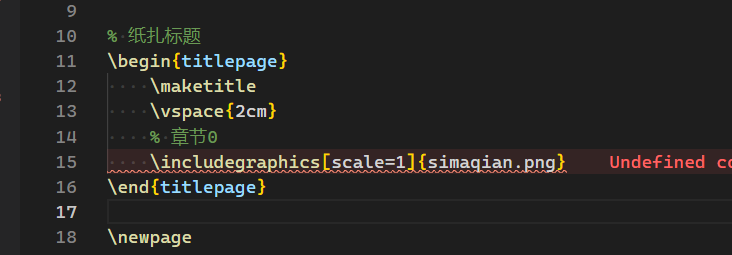
\includegraphics[scale=1.5]{simaqian.png}
\end{titlepage}
\end{lstlisting}


\subsection{如何使引用可以跳转?}
\label{sec:hyperreflink}

\subsubsection{操作}

一般情况下,我们希望目录是可以跳转的,图片的引用是可以鼠标点击跳转的。为了实现这个功能。我们可以使用$hyperref$。
操作方式:

1. 显示红框,可以点击:\verb!\usepackage{hyperref}!

2. 显示红色,可以点击:\verb!\usepackage[colorlinks=true]{hyperref}!

目录的内容显示为红色,是因为 hyperref 宏包的 colorlinks 选项。我们以后将默认载入这个宏包,告诉大家这些红色的文字都是可以点击跳转的,这也是我非常喜欢的一个特性。

当然也可以在配置里面进行配置。
\begin{lstlisting}[language=tex]
\hypersetup{
    colorlinks  = true,
    linkcolor   = blue,
    filecolor   = magenta,
    urlcolor    = cyan,
    pdftitle    = {Overleaf Example},
    pdfpagemode = FullScreen,
}
\end{lstlisting}

\subsubsection{注意事项}

1. 图、表建议添加"\verb!\label{标签}!"

2. 在需要添加引用的地方,输入"$\backslash$ref\{标签\}"

3. 之后就可以看到红色的引用标签了。

4. 如,$\backslash$ref\{sec:hyperreflink\}:\ref{sec:hyperreflink}

5. 如果只想引用不想点击,可以$\backslash$ref*\{sec:hyperreflink\}:\ref*{sec:hyperreflink}




\subsection{如何插入超链接?}

超链接分好几种。比如目录,比如图片引用等\ref{sec:hyperreflink}。

这里着重讨论其他外部连接。


\paragraph{Linking web addresses}
For further references see \href{http://www.overleaf.com}{Something Linky}
or go to the next url: \url{http://www.overleaf.com}

\begin{lstlisting}
For further references see \href{http://www.overleaf.com}{Something Linky}
or go to the next url: \url{http://www.overleaf.com}
\end{lstlisting}

\paragraph{Linking local files}
For further references see \href{http://www.overleaf.com}{Something Linky}
or go to the next url: \url{http://www.overleaf.com} or open the next
file \href{run:./file.txt}{File.txt}

\begin{lstlisting}
For further references see \href{http://www.overleaf.com}{Something Linky}
or go to the next url: \url{http://www.overleaf.com} or open the next
file \href{run:./file.txt}{File.txt}
\end{lstlisting}

\paragraph{Linking web addresses}


It's also possible to link directly any word
or \hyperlink{thesentence}{any sentence} in you document.

If you read this text, you will get no information.  Really?
Is there no information?

For instance \hypertarget{thesentence}{this sentence}.

这是一个文内的跳转方式。

\begin{lstlisting}
It's also possible to link directly any word
or \hyperlink{thesentence}{any sentence} in you document.

If you read this text, you will get no information.  Really?
Is there no information?

For instance \hypertarget{thesentence}{this sentence}.
\end{lstlisting}


\subsection{如何在 \LaTeX 中插入代码} % (fold)

\subsubsection{简单代码}
就像markdown一样,

1. 可以通过简单的\verb!`code`! 标记 来标识行内代码。

2. 通过进行多行显示原始代码。
\begin{verbatim}
            ```
            code
            code
            ```
        \end{verbatim}

\LaTeX 可使用原始显示的方式进行快速标识。虽然效果看不出来是行内代码,但是效果还是不错的,主要是字体稍微有点差别:\verb!这是code~!。

\begin{enumerate}
    \item 使用代码的$\backslash$verb!code!,进行简单的标识。但是中间不要太多“!” 号
    \item 使用 verbatim
          \begin{lstlisting}
        \begin{verbatim}
            code
        \end{verbatim}
            \end{lstlisting}

\end{enumerate}




\subsubsection{多行代码} % (fold)

% subsection  (end)
\begin{enumerate}
    \item usepackage Listings

          $\backslash$usepackage\{listingsutf8\}

    \item 设置代码的格式,暂时不错
    \item 在指定的位置插入一下例子
          \label{Code.Insert_pic}
          \begin{lstlisting}[language={tex}]
\begin{figure}[H] %H为当前位置,!htb为忽略美学标准,htbp为浮动图形
\centering %图片居中
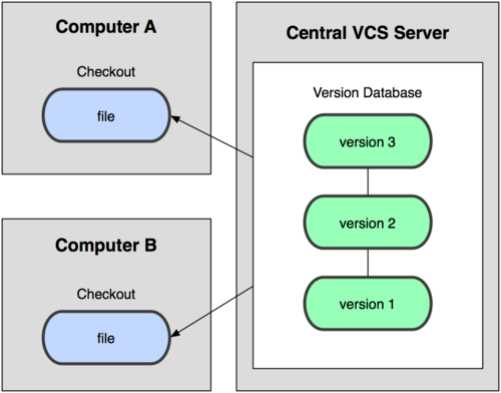
\includegraphics[width=0.7\textwidth]{images/svn-model.png}
%插入图片,[]中设置图片大小,{}中是图片文件名
\caption{集中化的版本控制系统} %最终文档中希望显示的图片标题
\label{Fig.main2} %用于文内引用的标签
\end{figure}
          \end{lstlisting}


\end{enumerate}

\begin{lstlisting}[language=c]
    void mian(int argl,string[] args){
        for(int i = 0;i<argl;)
            cout<<args[i]<<cendl;// 输出
    }
\end{lstlisting}

\subsection{如何在\LaTeX 中插入图片?}
\subsubsection{操作步骤}
插入图片是比较麻烦的时候。不像Word文档那样所见所得。

参考:https://blog.csdn.net/chichoxian/article/details/52588833

\begin{enumerate}
    \item 插入代码,参考代码\ref{Code.Insert_pic}
    \item 最终效果,图\ref{Fig.insert-one-png}
          \begin{figure}[H] %H为当前位置,!htb为忽略美学标准,htbp为浮动图形
              \centering %图片居中
              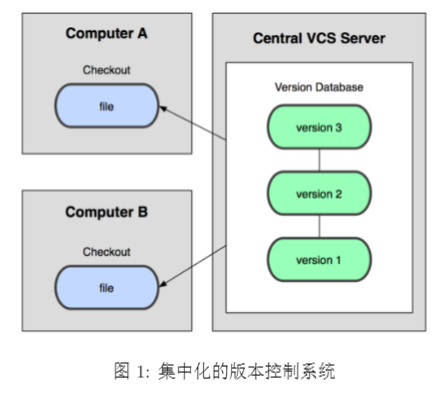
\includegraphics[width=0.5\textwidth]{images/insert-png.png} %插入图片,[]中设置图片大小,{}中是图片文件名
              \caption{插入图片的demo} %最终文档中希望显示的图片标题
              \label{Fig.insert-one-png} %用于文内引用的标签
          \end{figure}

    \item 双排设置
          \begin{lstlisting}
Figure \ref{Fig.main} has two sub figures, fig. \ref{Fig.sub.1} is the travel demand of driving auto, and fig. \ref{Fig.sub.2} is the travel demand of park-and-ride.

\begin{figure}[H]
\centering  %图片全局居中
\subfigure[name1]
{
    \label{Fig.sub.1}
    \includegraphics[width=0.45\textwidth]{DV_demand}
}
\subfigure[name2]
{
    \label{Fig.sub.2}
    \includegraphics[width=0.45\textwidth]{P+R_demand}
}
\caption{Main name}

\label{Fig.main}
\end{figure}
        \end{lstlisting}

    \item 双排效果显示,图 \ref{Fig.Insert_two_pic_demo}
          \begin{figure}[H]
              \centering
              %插入图片,[]中设置图片大小,{}中是图片文件名
              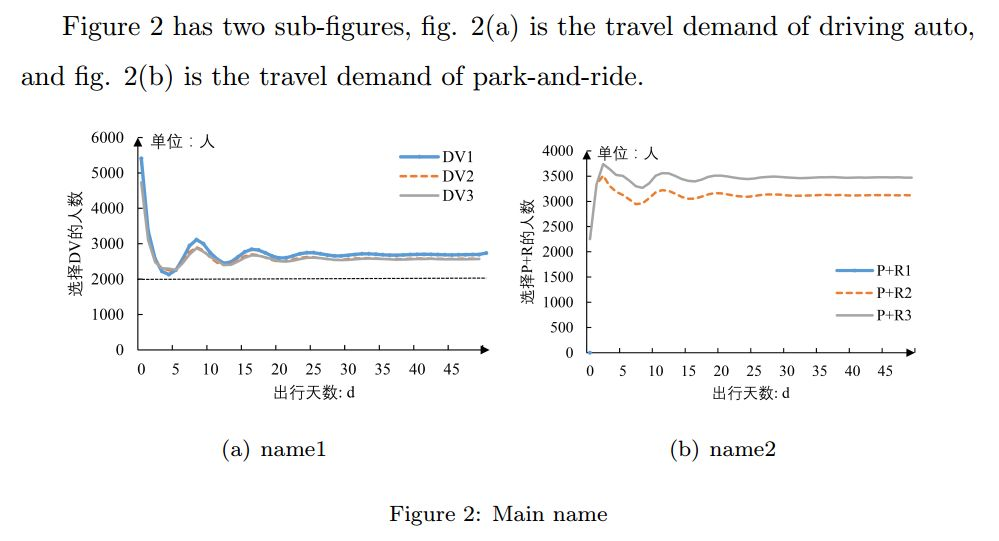
\includegraphics[width=1.0\textwidth]{images/insert-two-pic.jpg}
              \caption{并排插入两个图片的效果}
              \label{Fig.Insert_two_pic_demo}
          \end{figure}

    \item 引用图片

          在文档中使用$\backslash$ref\{标签\},如\verb!\ref{Fig.insert-one-png}!

\end{enumerate}








\subsection{如何设置边距}
\subsubsection{操作步骤}
\begin{enumerate}
    \item 引用geo 设置宏包
          $\backslash$usepackage\{geometry\}
    \item 设置页边距
          \begin{enumerate}
              \item 设置纸张大小

                    \verb!\geometry{papersize={20cm,15cm}}!
              \item 设置为缩放的形式

                    \verb!\geometry{a4paper,scale=0.8}!
              \item 设置为绝对距离

                    \verb!\geometry\{a4paper,left=2cm,right=2cm,top=2cm,bottom=2cm\}!
          \end{enumerate}
    \item 效果不错

\end{enumerate}


\subsubsection{页面边距设置概念}

\begin{figure}[H] %H为当前位置,!htb为忽略美学标准,htbp为浮动图形
    \centering %图片居中
    %插入图片,[]中设置图片大小,{}中是图片文件名
    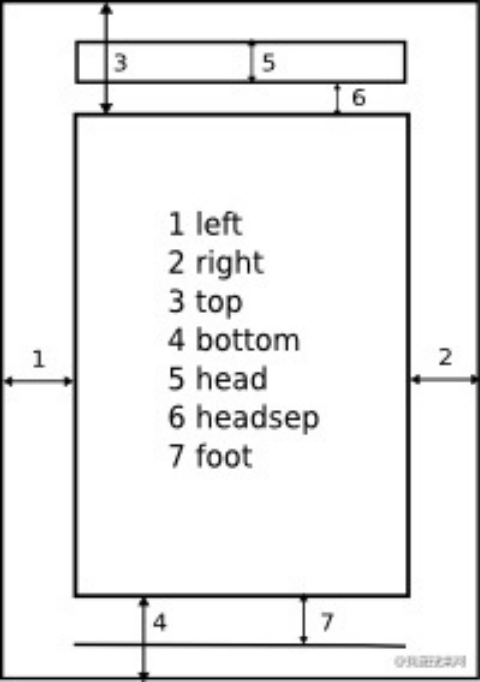
\includegraphics[scale=0.75]{images/geometry.png}
    \caption{页边距概念} %最终文档中希望显示的图片标题
    \label{Fig.page_border} %用于文内引用的标签
\end{figure}



\cprotect\subsection{如何输出反斜杠"\verb!\!"?}
要想打印 "\verb!\!" 比较麻烦。参考 https://blog.csdn.net/xovee/article/details/106728213
\begin{enumerate}
    \item 文本中

          \begin{enumerate}
              \item 使用"\verb!\!verb!\verb!\!!",注意是"!!" 之间进行截止
              \item 使用\verb!$\backslash$!
              \item 使用代码
                    \begin{lstlisting}{language=tex}
\usepackage{verbatim}
\begin{verbatim} % 使用代码的的形式显示
    \
\end{verbatim}
                    \end{lstlisting}
          \end{enumerate}

    \item 标题中

          1. 引用 cprotect 宏
          \begin{lstlisting}
\usepackage{cprotect}
% 在标题中显示原始字符
            \end{lstlisting}

          2. 在 标题中插入
          \begin{lstlisting}
\cprotect\section{This is a section heading with a verbatim \verb!\frac{1}{2}!}
% 这是在标题中使用\verb
          \end{lstlisting}

\end{enumerate}




\subsection{插入表格}

tabular环境提供了最简单的表格功能。它用\verb!\hline!命令表示横线,|表示竖线;用\&来分列,用\verb!\!来换行;每列可以采用居中、居左、居右等横向对齐方式,分别用l、c、r 来表示。

\subsubsection{操作步骤}
使用以下的代码。显示效果参考 表\ref{Table.Demo0}
\begin{lstlisting}{language=LaTeX}
\begin{table}[H]
    \centering
    \caption{论文中常用符号释义}
    \label{编译器}
    \begin{tabular}{|c|l|r|}
        \hline
        操作系统   & 发行版   & 编辑器    \\
        \hline
        Windows    & MikTeX   & TexMakerX \\
        % \hline
        Unix/Linux & teTeX    & Kile      \\
        % \hline
        Mac OS     & MacTeX   & TeXShop   \\
        % \hline
        通用       & TeX Live & TeXworks  \\
        \hline
    \end{tabular}

\end{table}
\end{lstlisting}

\subsubsection{效果显示}

\begin{table}[H]
    \centering
    \caption{表格demo}
    \label{Table.Demo0}
    \begin{tabular}{|c|l|r|}
        \hline
        操作系统   & 发行版   & 编辑器    \\
        \hline
        Windows    & MikTeX   & TexMakerX \\
        % \hline
        Unix/Linux & teTeX    & Kile      \\
        % \hline
        Mac OS     & MacTeX   & TeXShop   \\
        % \hline
        通用       & TeX Live & TeXworks  \\
        \hline
    \end{tabular}

\end{table}





% \begin{table}[H]
% \centering
% \caption{论文中常用符号释义\protect\footnotemark[1]}
%     \begin{tabular}{rl}
%     \hline
%     \multicolumn{1}{l}{符号} & 含义 \bigstrut\\
%     \hline
%         $\bm{p}$  & 充电器依次经历的节点号,即充电器的移动路径 \bigstrut[t]\\
%         $d(i,j)$ & 节点$i,j$之间的距离 \\
%     $T$& 充电器往返充电一次,所花费的时间 \\
%         $v$   & 充电器的移动速度 \\
%         $R_i$  & 节点$i$的耗电速率 \\
%         $r$  & 充电器的充电速率 \\
%         $t_{rtes}$  & 充电器在路上损耗的时间 \\
%         $t_{crg}$  & 充电器总的充电时间 \\
%         $W_i^\prime$  & 节点$i$在充电时刻的剩余电量 \\
%         $W_i$  & 节点$i$的电池容量 \\
%         $Q_i$  & 节点$i$当前时的剩余电量 \\
%         $\Delta t_i$  & 节点$i$充满电所需要的时间 \bigstrut[b]\\
%     \hline
%     \end{tabular}%
% \label{tab:addlabel}%

% \end{table}%
% \footnotetext[1]{这里只展示论文的部分符号。符号首次出现时,本文将详细地说明其含义}

\subsubsection{居中}
有时候,用 \verb!\begin{center}-\end(center}! 来将表格整体居中,但它的居中只是 居中了 \verb!\begin{table}-\end{table}!;如果\verb!\begin{table}-\end{table}! 里面嵌套了 \verb!\begin{tabular}-\end{tabular}! ,那么表格还是不会居中。要使得表格居中,则需要在 \verb!\begin{table}! 后面附加 \verb!\centering!,才能使得表格整体居中。



\newpage
\section{\LaTeX 高级技巧}
\subsection{我们如何知道需要引用什么宏呢?}
当我们需要用什么东西的时候,我们该如何知道要引用什么?
比如我们要用超链接,我们就需要引用 hyperref 这个宏包?那我该如何知道呢?

% \usepackage{bbding}
% \usepackage{pifont}
% \usepackage{wasysym}
% \usepackage{amssymb}


% amssymb
\checkmark

% bbding
\Checkmark
\CheckmarkBold

% pifont
\ding{51}
\ding{52}

% wasysym
\CheckedBox




\subsection{如何对宏进行配置?}
当我们引用一个宏的时候,我们如何知道怎么配置这个宏呢?
比如我们引用 hyperref 宏的时候。我是如何知道我可以配置一下的这些东西呢?

\begin{lstlisting}
\hypersetup{
    colorlinks  = true,
    linkcolor   = blue,
    filecolor   = magenta,
    urlcolor    = cyan,
    % pdftitle    = {Overleaf Example},
    % pdfpagemode = FullScreen,
}
\end{lstlisting}




\end{document}